%% End-semester report in the IIIT Allahabad B.Tech thesis format (btech_Template.pdf).
%% Extends the mid-term report with Chapters 6-8 (extended benchmarks, garbage collection, correctness proof).
%% Build:  tectonic -X compile main.tex   (XeTeX; fonts are loaded from ./fonts, copies of C:/Windows/Fonts files; no biber needed)
\documentclass[11pt,a4paper,oneside]{report}

% ---------------------------------------------------------------- fonts (Palatino-style, as in the template)
\usepackage{mathpazo}
\usepackage[no-math]{fontspec}
\setmainfont{texgyrepagella}[Extension=.otf, UprightFont=*-regular, BoldFont=*-bold, ItalicFont=*-italic, BoldItalicFont=*-bolditalic]
\setmonofont{consola.ttf}[Path=./fonts/, Scale=0.9, BoldFont=consolab.ttf, ItalicFont=consolai.ttf,
  BoldItalicFont=consolaz.ttf]
\newfontfamily\hindifont{Nirmala.ttc}[Path=./fonts/, FontIndex=0, BoldFont=Nirmala.ttc,
  BoldFeatures={FontIndex=1}, Script=Devanagari]

% ---------------------------------------------------------------- page layout
\usepackage[a4paper, top=2.6cm, bottom=2.6cm, left=2.5cm, right=2.1cm, headheight=15pt]{geometry}
\usepackage{setspace}
\setstretch{1.7}
\setlength{\parindent}{0pt}
\setlength{\parskip}{6pt}

\usepackage{graphicx}
\usepackage{booktabs}
\usepackage{makecell}
\usepackage{amssymb}
\usepackage{array}
\usepackage{float}
\usepackage{enumitem}
\setlist{itemsep=1pt, topsep=3pt}
\newcolumntype{P}[1]{>{\raggedright\arraybackslash}p{#1}}
\usepackage{xcolor}
\usepackage{tikz}
\usetikzlibrary{arrows.meta,positioning,calc}
\usepackage{pgfplots}
\pgfplotsset{compat=1.18}
\usepackage[hidelinks]{hyperref}

\definecolor{cGTX}{HTML}{1F5FA8}
\definecolor{cCONS}{HTML}{7AA6D6}
\definecolor{cHUB}{HTML}{C02D2D}
\definecolor{cHUBL}{HTML}{E69A9A}
\definecolor{cGRN}{HTML}{1B7F5E}
\definecolor{cORG}{HTML}{C8651B}
\definecolor{iiitblue}{HTML}{1F3FA8}

% ---------------------------------------------------------------- headers / footers: "Chapter N. Title" + [page]
\usepackage{fancyhdr}
\pagestyle{fancy}
\fancyhf{}
\renewcommand{\chaptermark}[1]{\markboth{\textit{\chaptername\ \thechapter.\ #1}}{}}
\fancyhead[L]{\leftmark}
\fancyfoot[C]{[\thepage]}
\renewcommand{\headrulewidth}{0.4pt}
\fancypagestyle{plain}{\fancyhf{}\fancyfoot[C]{[\thepage]}\renewcommand{\headrulewidth}{0pt}}
\fancypagestyle{front}{\fancyhf{}\fancyfoot[C]{[\thepage]}\renewcommand{\headrulewidth}{0pt}}

% ---------------------------------------------------------------- report data
\newcommand{\ttitle}{Contention-Aware Transactions for Dynamic Graph Updates on GPUs}
\newcommand{\sys}{GTX-GPU}
\newcommand{\code}[1]{\texttt{#1}}

\begin{document}
\hypersetup{pageanchor=false}

%% ================================================================ TITLE PAGE
\begin{titlepage}
\begin{singlespace}
\begin{center}
\vspace*{0.6cm}
{\LARGE\bfseries \ttitle\par}
\vspace{1.1cm}
{\small\itshape A thesis submitted in partial fulfillment of the requirements\\ for the award of the degree of\par}
\vspace{0.8cm}
{\LARGE BACHELOR OF TECHNOLOGY\par}
\vspace{0.4cm}

\includegraphics[width=4.3cm]{college.jpg}\par
\vspace{0.9cm}
\begin{singlespace}
\begin{minipage}[t]{0.48\textwidth}
\raggedright
\textit{By:-}\\[2pt]
\textsc{Suyash Kumar}\\
\textsc{Vivek G Nair}\\
\textsc{Aryan Pandey}
\end{minipage}\hfill
\begin{minipage}[t]{0.48\textwidth}
\raggedleft
\textit{Enrollment No.}\\[2pt]
IIT2024169\\
IIT2024125\\
IIT2024128
\end{minipage}
\end{singlespace}
\vspace{0.7cm}
{\small\itshape Under the Supervision of\par}
{\large \textsc{Dr. Anshu S Anand}\par}
\vspace{0.5cm}
{\small\itshape Submitted to the\par}
{\large \textsc{Department of Information Technology}\par}
\vspace{0.7cm}
{\large\hindifont भारतीय सूचना प्रौद्योगिकी संस्थान, इलाहाबाद\par}
\vspace{0.1cm}
{\large \textsc{Indian Institute of Information Technology,}\\ \textsc{Allahabad}\par}
\vspace{0.9cm}
{\small November 2026\par}
\end{center}
\end{singlespace}
\end{titlepage}

%% ================================================================ CERTIFICATE (letterhead)
\pagenumbering{roman}
\setcounter{page}{1}
\thispagestyle{empty}
\begin{singlespace}
\noindent
\begin{minipage}[c]{2.6cm}

\includegraphics[width=2.5cm]{college.jpg}
\end{minipage}%
\begin{minipage}[c]{\dimexpr\textwidth-2.6cm\relax}
\centering
{\large\bfseries\color{iiitblue}\hindifont भारतीय सूचना प्रौद्योगिकी संस्थान इलाहाबाद\par}
{\Large\bfseries\color{iiitblue} Indian Institute of Information Technology Allahabad\par}
{\small\bfseries An Institute of National Importance by Act of Parliament\par}
{\small Deoghat Jhalwa, Prayagraj 211015 (U.P.) India\par}
{\scriptsize Ph: 0532-2922025, 2922067; Web: www.iiita.ac.in; Email: contact@iiita.ac.in\par}
\end{minipage}
\par\vspace{2pt}\noindent\rule{\textwidth}{0.6pt}
\end{singlespace}

\vspace{1.2cm}
\begin{center}{\large\bfseries CERTIFICATE}\end{center}
\vspace{0.3cm}
It is certified that the work contained in the thesis titled ``\ttitle'' by Suyash Kumar, Vivek G Nair, Aryan Pandey
has been carried out under my supervision and that this work has not been submitted elsewhere for a degree.

\vspace{3cm}
\hfill
\begin{minipage}{0.42\textwidth}
\begin{singlespace}
\noindent\rule{\textwidth}{0.3pt}\\
Dr. Anshu S Anand\\
Department of Information Technology\\
IIIT Allahabad
\end{singlespace}
\end{minipage}
\clearpage

%% ================================================================ CANDIDATE DECLARATION
\thispagestyle{empty}
\begin{center}{\large\bfseries CANDIDATE DECLARATION}\end{center}
We, Suyash Kumar (IIT2024169), Vivek G Nair (IIT2024125), and Aryan Pandey (IIT2024128), hereby
certify that the thesis titled ``\ttitle'' has been submitted by us in partial fulfillment of the requirements for the
Degree of Bachelor of Technology in the Department of Information Technology at the Indian Institute of Information
Technology, Allahabad.

We acknowledge that plagiarism includes:
\begin{enumerate}
\item Reproducing another person's work (fully or partially) or ideas and presenting them as our own.
\item Copying or paraphrasing another person's work without appropriate attribution.
\item Engaging in literary theft by reproducing a unique literary construct without crediting its source.
\end{enumerate}
We affirm that due credit has been given to all original authors and sources through proper citations for words,
ideas, diagrams, graphics, computer programs, experiments, results, and websites that are not our own contributions.
Direct quotations have been appropriately marked, and sources have been properly referenced. Furthermore, we declare
that no portion of our work is plagiarized. In the event of a plagiarism claim, we accept full responsibility for the
contents of this thesis. We acknowledge that our supervisor may not be able to verify the originality of every aspect
of our work.

\vspace{0.6cm}
\begin{singlespace}
\noindent
\begin{minipage}[t]{0.45\textwidth}
Place:\\[6pt]
Date:
\end{minipage}\hfill
\begin{minipage}[t]{0.45\textwidth}
\raggedleft
Suyash Kumar (IIT2024169)\\[16pt]
Vivek G Nair (IIT2024125)\\[16pt]
Aryan Pandey (IIT2024128)
\end{minipage}
\end{singlespace}
\clearpage

%% ================================================================ ABSTRACT
\pagestyle{front}
\thispagestyle{front}
\begin{center}
{\normalsize INDIAN INSTITUTE OF INFORMATION TECHNOLOGY, ALLAHABAD\par}
\vspace{0.3cm}
{\large\bfseries \ttitle\par}
\vspace{0.3cm}
{\large ABSTRACT\par}
\end{center}
\addcontentsline{toc}{chapter}{Abstract}
On a GPU thousands of threads update a dynamic graph at once, and in skewed real graphs many updates converge on a few
hub vertices, where unsynchronised updates corrupt state and locks destroy throughput. Generic GPU software
transactional memories ignore graph structure, while GPU dynamic-graph systems apply batched updates without
transactions. This report presents \sys{}, which keeps the architecture of GTX, a transactional dynamic-graph system for
CPUs, and redesigns four mechanisms for GPU (SIMT) execution: (1)~every change is a new version, (2)~storage grows by
linking larger blocks instead of copying, (3)~a warp reserves space with a single atomic operation, and (4)~writers use
lock-free check-then-swap with conflicts detected per edge. On an RTX~4060 Laptop GPU it sustains 140--180 million
edge inserts per second, with no false aborts (45\% to 0\% at 32 edges per transaction).

This end-semester report extends that work in three directions. First, \sys{} is compared with two-phase locking,
a TL2-style STM and GPMA+ on identical streams, including concurrent snapshot readers, a new serializable mode and four
real graphs: it is one to four orders of magnitude faster where updates concentrate on hubs or readers scan the graph
(for example 19.9--20.6$\times$ with 90\% readers), faster than GPMA+ at every batch size (1.8--16.5$\times$) and
on every real graph stream, and 0.37--0.84$\times$ of locking on uniform graphs without contention. Second, garbage
collection: a compaction between kernel launches keeps memory flat over long update streams, at 0.70--0.81$\times$ of
throughput on write-heavy streams. Third, a paper proof against the GPU memory model shows that every history satisfies snapshot
isolation (and serializability in the serializable mode); writing it found two ordering defects that no test had
observed, and a correctness gate of 219 test cases exercises it.

\vspace{0.2cm}
\textbf{Keywords:} Dynamic graph, GPU, transactions, software transactional memory, multi-versioning, lock-free
synchronisation
\clearpage

%% ================================================================ LISTS
\begin{singlespace}
\tableofcontents
\clearpage
\addcontentsline{toc}{chapter}{List of Figures}
\listoffigures
\clearpage
\addcontentsline{toc}{chapter}{List of Tables}
\listoftables
\clearpage
\chapter*{List of Abbreviations}
\addcontentsline{toc}{chapter}{List of Abbreviations}
\begin{tabular}{@{}p{2.6cm}l@{}}
2PL & Two-Phase Locking \\
CAS & Compare-And-Swap \\
CPU & Central Processing Unit \\
DSTM & Dynamic Software Transactional Memory \\
GPU & Graphics Processing Unit \\
PTX & Parallel Thread Execution (NVIDIA's GPU instruction set and memory model) \\
SER & Serializable (isolation level) \\
SI & Snapshot Isolation \\
SIMT & Single Instruction, Multiple Threads \\
SNAP & Stanford Network Analysis Project (graph collection) \\
STM & Software Transactional Memory \\
TL2 & Transactional Locking II (a software transactional memory) \\
\end{tabular}
\end{singlespace}
\clearpage

%% ================================================================ MAIN MATTER
\pagenumbering{arabic}
\pagestyle{fancy}
\hypersetup{pageanchor=true}

%% ---------------------------------------------------------------------------------------------------- Chapter 1
\chapter{Introduction}
\label{ch:intro}
This chapter introduces dynamic graphs, the research question that motivates this work, and the contributions of this
report, and describes how the remaining chapters are organised.

\section{Dynamic Graphs}
A \emph{dynamic graph} $G(t) = (V(t), E(t))$ is a graph whose vertex and edge sets change over time through insertions
and deletions. A static graph is built once and then analysed; a dynamic graph is updated continuously as new data
arrives, for example when friendships are formed in a social network or roads are closed in a road network. Typical
examples are social networks, road networks, communication networks and recommendation graphs.

\section{Research Question}
GPUs are an attractive platform for dynamic graphs because they process many edge updates at once. The difficulty is
that every GPU thread must safely access the same changing graph. Many real updates also come in groups that only make
sense together, such as a user switching from following account A to following account B (delete one edge, insert
another). This leads to our research question:
\begin{quote}
\emph{How can thousands of GPU threads update a shared dynamic graph concurrently while preserving correctness and
performance?}
\end{quote}

\section{Contributions}
This report presents the project:
\begin{itemize}
\item the problem analysis: why concurrent updates, GPU execution and power-law skew make the problem hard
  (Chapter~\ref{ch:problem}), and the gap left by existing work (Chapter~\ref{ch:lit});
\item the proposed framework \sys{}, which adapts GTX~\cite{gtx} to the GPU through four ideas: versions instead of
  overwrites, storage growth without copying, one atomic operation per warp, and lock-free per-edge check-then-swap
  (Chapter~\ref{ch:framework});
\item preliminary benchmarks of the engine: throughput as transactions grow, abort ratio against GTX's original
  conflict rule, and mixed read/write transactions (Chapter~\ref{ch:eval});
\item an extended evaluation against locking, STM, non-transactional and batch-update baselines, with snapshot
  readers, a serializable mode and real graphs (Chapter~\ref{ch:exteval});
\item garbage collection of old versions by compaction between kernel launches, which keeps memory bounded over
  long update streams (Chapter~\ref{ch:gc});
\item a correctness proof of snapshot isolation and serializability against the GPU memory model, and the extended
  correctness tests (Chapter~\ref{ch:proof}).
\end{itemize}
Chapter~\ref{ch:conclusion} lists the future work and concludes.

%% ---------------------------------------------------------------------------------------------------- Chapter 2
\chapter{Problem Statement}
\label{ch:problem}
This chapter explains why concurrent updates to a shared graph are a problem, why GPU execution makes the problem both
attractive and hard, and how the power-law skew of real graphs concentrates contention on a few hub vertices.

\section{Why Concurrent Updates Are a Problem}
Consider multiple threads applying updates concurrently, many of them targeting the same vertex $A$: T1 inserts $(A,E)$,
T2 deletes $(A,B)$, T3 inserts $(A,F)$, T4 inserts $(A,G)$, T5 deletes $(A,C)$, and so on, all against one shared
adjacency structure. Without synchronisation this causes:
\begin{itemize}
\item \textbf{race conditions}: concurrent modification of shared state;
\item \textbf{lost updates}: one update overwrites another;
\item \textbf{inconsistent state}: the result does not reflect the requested updates;
\item \textbf{corruption}: structural invariants are violated.
\end{itemize}

When updates come in groups, a reader can also observe a group half done. Figure~\ref{fig:torn} shows such a
\emph{torn read}: a writer switches a user from following A to following B, and a reader that looks between the two
steps sees the user following nobody, a state that should never exist. Two guarantees are therefore needed:
\emph{all-or-nothing groups of changes} (transactions) and \emph{consistent reading during updates}.

\begin{figure}[H]
\centering
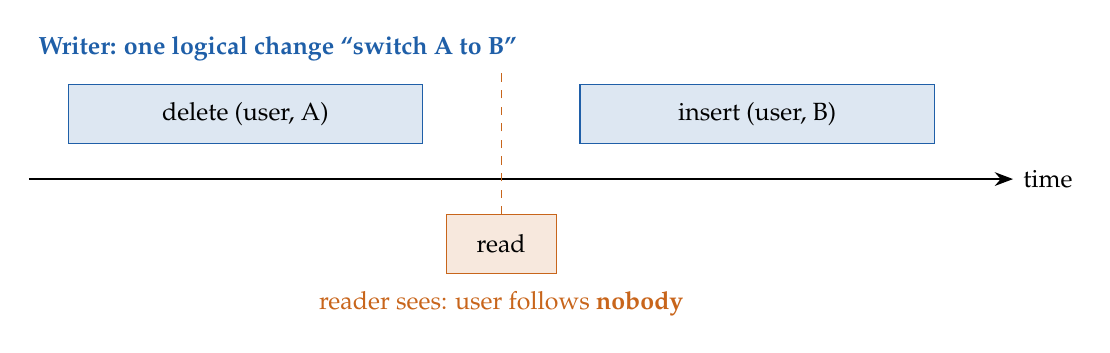
\begin{tikzpicture}[font=\small, >=Stealth]
\draw[->, thick] (0,0) -- (12.5,0) node[right] {time};
\draw[fill=cGTX!15, draw=cGTX] (0.5,0.45) rectangle (5.0,1.2) node[midway] {delete (user, A)};
\draw[fill=cGTX!15, draw=cGTX] (7.0,0.45) rectangle (11.5,1.2) node[midway] {insert (user, B)};
\node[cGTX, anchor=west] at (0,1.65) {\textbf{Writer: one logical change ``switch A to B''}};
\draw[fill=cORG!15, draw=cORG] (5.3,-1.2) rectangle (6.7,-0.45) node[midway] {read};
\draw[dashed, cORG] (6.0,-0.45) -- (6.0,1.4);
\node[cORG, align=center, anchor=north] at (6.0,-1.3) {reader sees: user follows \textbf{nobody}};
\end{tikzpicture}
\caption{A torn read: without transactions, a reader can observe half of a group of changes.}
\label{fig:torn}
\end{figure}

\section{Why GPUs, and Why This Is Hard}
GPUs execute in SIMT fashion: thousands of threads are grouped into \emph{warps} of 32 threads on NVIDIA GPUs, and the
threads of a warp execute the same instruction at the same time. Concurrent graph updates on a GPU therefore face race
conditions, warp divergence, deadlock or livelock, and synchronisation overhead, with symptoms such as lost updates,
duplicate edges and torn or inconsistent reads.

Graph processing is \emph{memory-bound}: irregular neighbour lookups and pointer chasing perform very little
computation per byte loaded, so memory bandwidth sets the speed limit. This favours the GPU. On data-centre hardware,
the peak memory bandwidth of an NVIDIA H100 (HBM3) is 3.35~TB/s against about 0.31~TB/s for an Intel Xeon socket with
DDR5, roughly 11$\times$ higher, which keeps thousands of GPU threads fed with graph data; while some warps wait for
memory, the GPU runs others. (Our own experiments run on an RTX~4060 Laptop GPU.)

The challenge is therefore not just parallelism but preserving correctness and progress while many GPU threads update
shared graph state concurrently. Locks can be effective at low contention, but under massive GPU parallelism they
serialise access and can destroy throughput.

\section{Motivation: Power-Law Skew and Hub Contention}
Real graphs are highly skewed: a small fraction of vertices account for a disproportionate share of connectivity and
updates (heavy-tailed, power-law behaviour: few hubs, many low-degree vertices). Parallel insertions and deletions
therefore repeatedly access the adjacency data of the same high-degree vertex, and that shared state becomes the
bottleneck: synchronisation pressure causes retries, serialisation, heavy atomic traffic and lower throughput. Massive
parallelism does not guarantee scalable updates when many threads converge on the same shared graph structure; the
challenge is to preserve correctness and throughput under highly skewed update streams.

%% ---------------------------------------------------------------------------------------------------- Chapter 3
\chapter{Literature Review}
\label{ch:lit}
This chapter reviews software transactional memory and dynamic graph processing on GPUs, describes GTX, the CPU system
on which our framework is based, and states the research gap.

\section{Software Transactional Memory}
Table~\ref{tab:stm} summarises the transactional-memory work we build on. STM~\cite{stm} introduced transactions as a
higher-level concurrency abstraction that provides atomicity and consistency without explicit lock management.
DSTM~\cite{dstm} extended STM to dynamically sized data structures. GPU-STM~\cite{gpustm} showed that STM is feasible
on GPUs, and CSMV~\cite{csmv} showed that GPU STM can be optimised further with a multi-versioned, client-server design.

\textbf{Issue.} These are generic STMs: they do not exploit exact graph semantics or distinguish structural contention
from true edge-level conflicts, and their read/write tracking, validation and transaction management can add
non-trivial overhead for fine-grained graph updates. For example, every insert into a popular vertex also updates that
vertex's edge counter, so unrelated transactions collide on that single word.

\begin{table}[H]
\caption{Software transactional memory.}
\label{tab:stm}
\small
\begin{singlespace}
\begin{tabular}{@{}P{2.6cm}P{3.9cm}P{4.6cm}P{3.6cm}@{}}
\toprule
Work & Core contribution & Key idea & What it gives us \\
\midrule
STM (PODC 1995)~\cite{stm} & Introduces STM as a higher-level concurrency abstraction & Transactions provide atomicity and consistency without explicit lock management & Separates application logic from synchronisation \\
DSTM (PODC 2003)~\cite{dstm} & Extends STM to dynamically sized data structures & Dynamic read/write tracking; demonstrated with red-black trees & Relevant to dynamically changing structures \\
GPU-STM (CGO 2014)~\cite{gpustm} & Adapts STM to GPU architectures & Hierarchical validation and encounter-time lock sorting & Shows STM is feasible on GPUs \\
CSMV (IPDPS 2022)~\cite{csmv} & Multi-version GPU STM & Client-server design separates execution from commit processing & Shows GPU STM can be further optimised \\
\bottomrule
\end{tabular}
\end{singlespace}
\end{table}

\section{Dynamic Graph Processing on GPUs}
Table~\ref{tab:dg} summarises dynamic-graph work. GPMA and GPMA+~\cite{gpma} process batches of dynamic updates on the
GPU using a packed-memory array. Hornet~\cite{hornet} provides a dynamic sparse-graph structure for GPUs with a
hierarchical representation and dynamic memory management. The survey of Gao et al.~\cite{survey} gives a taxonomy of
representations, updates and analytics. These systems apply updates batch at a time; none offers groups of changes that
are all-or-nothing, or safe reading while updates run.

\textbf{Takeaway.} Existing systems optimise dynamic graph updates, but transactional semantics and GPU-specific,
graph-aware concurrency remain largely separate.

\begin{table}[H]
\caption{Dynamic graph processing.}
\label{tab:dg}
\small
\begin{singlespace}
\begin{tabular}{@{}P{2.9cm}P{3.9cm}P{4.5cm}P{3.4cm}@{}}
\toprule
Work & Core contribution & Key idea & What it gives us \\
\midrule
GPMA / GPMA+ (PVLDB 2017)~\cite{gpma} & GPU batches of dynamic updates & Packed-memory array for GPU parallelism & Strong specialised baseline \\
Hornet (HPEC 2018)~\cite{hornet} & Dynamic sparse graph for GPUs & Hierarchical representation and dynamic memory management & Need for specialised structures \\
GTX (PACMMOD 2025)~\cite{gtx} & Write-optimised, transactional graph system (CPU) & Adaptive delta-chain locking; no vertex locks; group commit & Closest related; motivates exact-edge conflicts on GPU \\
Survey (FCS 2024)~\cite{survey} & Taxonomy of GPU dynamic graphs & Representations, updates, analytics & Places the problem in the field \\
\bottomrule
\end{tabular}
\end{singlespace}
\end{table}

\section{GTX}
GTX~\cite{gtx} is a transactional dynamic-graph system for CPUs. Four of its ideas are the basis of our framework:
\begin{enumerate}
\item \emph{versions instead of overwrites}: every change to an edge is stored as a new version with timestamps, so
  readers look at old versions while writers add new ones and readers never wait for writers;
\item \emph{delta chains}: the versions of edges are linked in chains, so a writer can quickly check whether someone else
  is changing the same data;
\item \emph{status lookup on demand}: a version records which transaction wrote it, and a reader checks that
  transaction's status (running, committed, aborted) only when it meets the version;
\item \emph{group commit}: transactions commit in numbered batches.
\end{enumerate}
GTX takes a lock bit on a whole delta chain to detect write--write conflicts, so conflicts are judged per chain, and it
copies a full edge block into a larger one when it fills up.

\section{Research Gap}
GTX demonstrates a transactional dynamic-graph system on CPUs. Our question is whether the same kind of general
transactional graph-update abstraction can be achieved on GPUs, while redesigning the concurrency mechanisms for GPU
(SIMT) execution and severe skew. A direct port does not work: the 32 threads of a warp often target the same hub
vertex, so per-thread atomics on that vertex serialise and a thread waiting for a lock inside a warp can block the
thread that holds it; a full block cannot be copied while thousands of threads may be writing into it; and
memory-ordering bugs on a GPU are silent, producing rare wrong reads rather than crashes. Our goal is to keep GTX's
architecture and redesign exactly the parts the GPU breaks.

%% ---------------------------------------------------------------------------------------------------- Chapter 4
\chapter{Proposed Framework: GTX-GPU}
\label{ch:framework}
This chapter presents the architecture of \sys{}, its four GPU-specific ideas, how lookups, scans and commits work, how
correctness is validated, and how the design differs from GTX.

\section{Architecture Overview}
Figure~\ref{fig:arch} shows the whole system. It has three parts:
\begin{enumerate}
\item \textbf{Per-vertex arrays} (left). Each vertex $u$ has two entries. \code{vcur[u]} holds the id of $u$'s current
  (newest) storage block and is used by readers to know where to start. \code{vfill[u]} is a single 64-bit reservation
  word used by writers: its high half is the block (generation) and its low half is the number of slots already taken
  in that block. In the figure, vertex~2 has \code{vfill} $=(g\,|\,37)$: its current block is $g$ and the next writer
  receives slot~37.
\item \textbf{Block generations with delta chains} (middle). Each block has a row of \emph{records} (one per change;
  ``7\,I'' means \emph{edge to vertex 7 inserted}, ``7\,D'' \emph{deleted}, V a reserved slot left unused) and a row of
  \emph{chain heads}, entry points that point at the newest record of the edges hashed to them. The \emph{prev} links
  connect older versions of the same edge; for destination 7 the chain is 7D $\rightarrow$ 7I $\rightarrow$ 7I in the
  older block. The older block $g{-}1$ is still read but never copied; S marks a sealed chain head.
\item \textbf{Version record and transaction status} (right): the layout of one record, and the table of transaction
  states that readers consult.
\end{enumerate}

\begin{figure}[H]
\centering
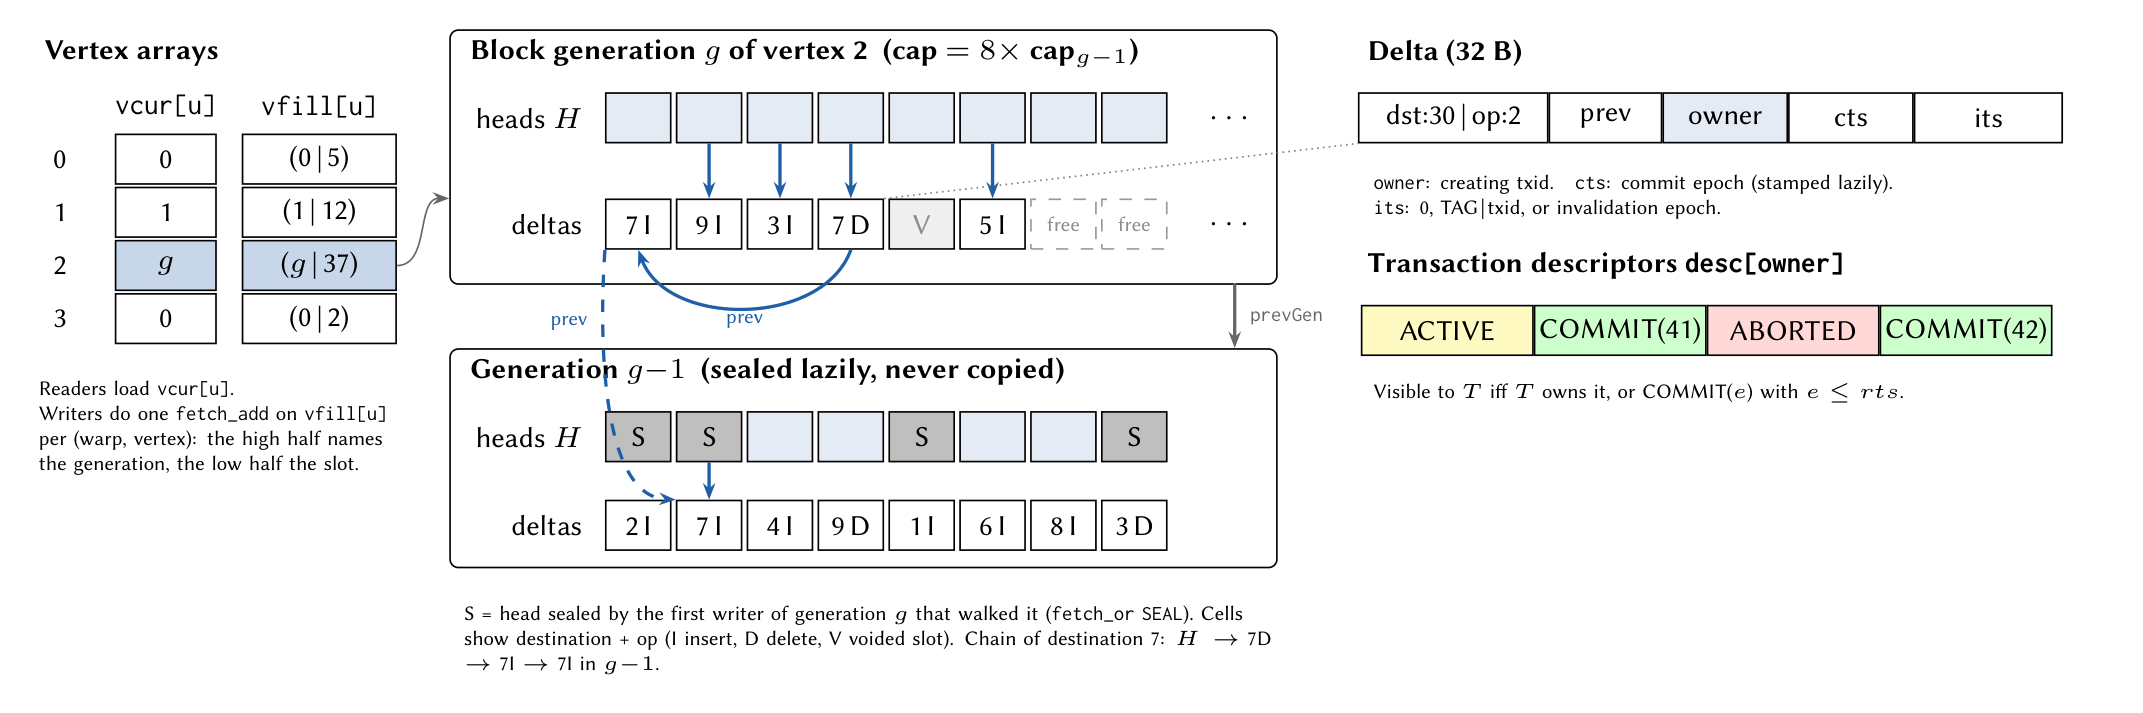
\includegraphics[width=\textwidth]{arch_fw.png}
\caption{\sys{} architecture. Left: per-vertex arrays (current block, and one reservation word holding block and slots
used). Middle: the storage blocks of vertex 2, newest first; each record is one version of an edge; versions of the
same edge are linked in a chain; S marks a chain sealed in the older block. Right: the 32-byte version record and the
transaction status table.}
\label{fig:arch}
\end{figure}

\section{Idea 1: Every Change Is a New Version}
Nothing is overwritten: an insert or a delete appends a small record (32 bytes) with five fields
(Table~\ref{tab:record}). The state of an edge, for a given reader, is the \emph{newest version that reader is allowed
to see}: its own version, or one whose writer committed before the reader started. A delete is a new record, not an
erase.

\begin{table}[H]
\caption{Fields of one version record (32 bytes).}
\label{tab:record}
\small
\begin{singlespace}
\begin{tabular}{@{}P{2.2cm}P{12.8cm}@{}}
\toprule
Field & Meaning \\
\midrule
\code{dst\,|\,op} & which edge (destination vertex) and whether it is an insert or a delete \\
\code{prev} & the previous version of the same edge (the chain link) \\
\code{owner} & the transaction that wrote it \\
\code{cts} & commit time, filled in after commit \\
\code{its} & invalidation time: 0 while the edge is present; while a running transaction is deleting it, a tag with
  that transaction's id; afterwards the deletion's commit time \\
\bottomrule
\end{tabular}
\end{singlespace}
\end{table}

Figure~\ref{fig:chain} shows three versions of edge $(u,7)$, newest first. A reader that started at time~7 walks newest
to oldest: it skips T3 (not committed), skips T2 (committed at 9, after it started) and uses T1, so the edge is
\emph{present}. A reader that started at time~10 uses T2 and sees the edge \emph{absent}. Different readers see
different but always consistent states. Two consequences follow: readers never wait for writers, because they simply
skip versions that are too new; and an aborted transaction needs no rollback, because its versions stay invisible
forever.

The \code{prev} chain serves point lookups of one edge, while \code{its} serves scans: a scan reads a vertex's records
slot by slot, and \code{its} tells it immediately whether an insert was deleted before the reader started.

\begin{figure}[H]
\centering
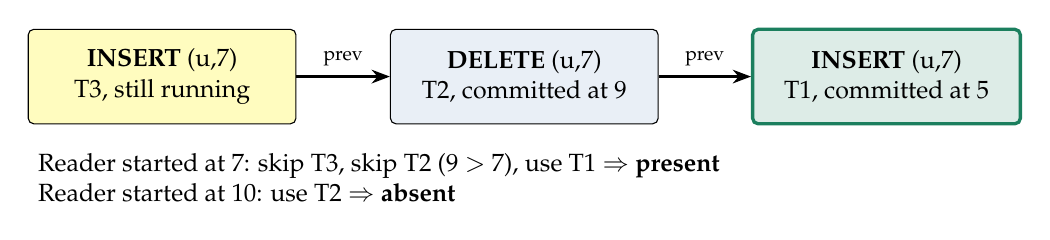
\begin{tikzpicture}[font=\small, >=Stealth,
  ver/.style={draw, rounded corners=2pt, minimum width=3.4cm, minimum height=1.2cm, align=center}]
\node[ver, fill=yellow!25] (v3) at (0,0) {\textbf{INSERT} (u,7)\\ T3, still running};
\node[ver, fill=cGTX!10] (v2) at (4.6,0) {\textbf{DELETE} (u,7)\\ T2, committed at 9};
\node[ver, fill=cGRN!15, very thick, draw=cGRN] (v1) at (9.2,0) {\textbf{INSERT} (u,7)\\ T1, committed at 5};
\draw[->, thick] (v3) -- node[above, font=\scriptsize] {prev} (v2);
\draw[->, thick] (v2) -- node[above, font=\scriptsize] {prev} (v1);
\node[align=left, anchor=north west] at (-1.7,-0.85) {Reader started at 7: skip T3, skip T2 (9 $>$ 7), use T1 $\Rightarrow$ \textbf{present}\\
Reader started at 10: use T2 $\Rightarrow$ \textbf{absent}};
\end{tikzpicture}
\caption{Three versions of one edge and what two readers see.}
\label{fig:chain}
\end{figure}

\section{Idea 2: Storage Grows Without Copying}
When a vertex's block fills up, thousands of GPU threads may still be writing into it, so it is never copied
(Figure~\ref{fig:grow}):
\begin{enumerate}
\item the one thread whose slot number equals the block's capacity becomes the \emph{grower};
\item it allocates a block 8$\times$ larger and links it in front of the old one;
\item it publishes the new block (\code{vcur}, then \code{vfill}); waiting threads retry and land in it;
\item the old block stays readable. The first writer that walks an edge's chain into the old block \emph{seals} that
  chain there (sets a SEAL bit on its head), so from then on that edge's new versions go only to the newest block.
\end{enumerate}
Sealing is done lazily, chain by chain, by the first writer that needs it, so no thread ever has to stop, and all
versions of one edge stay in a single order. Growing by a large factor makes growth rare.

\begin{figure}[H]
\centering
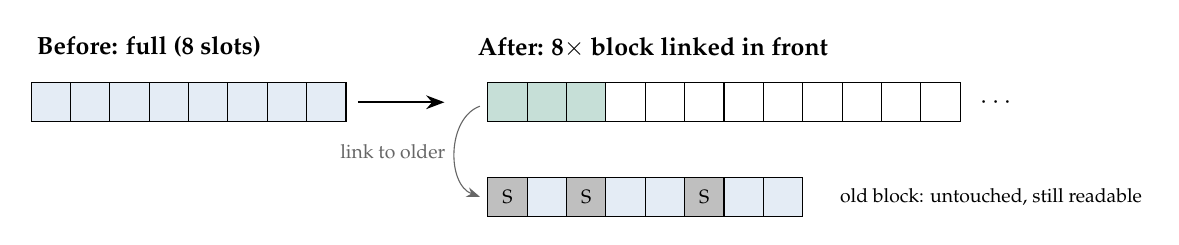
\begin{tikzpicture}[font=\small, >=Stealth, s/.style={draw, minimum width=0.5cm, minimum height=0.5cm, inner sep=0pt}]
\node[anchor=west] at (-0.3,1.3) {\textbf{Before: full (8 slots)}};
\foreach \i in {0,...,7} \node[s, fill=cGTX!12] at (\i*0.5,0.6) {};
\draw[->, thick] (3.9,0.6) -- (5.0,0.6);
\node[anchor=west] at (5.3,1.3) {\textbf{After: 8$\times$ block linked in front}};
\foreach \i in {0,...,11} \node[s, fill=white] at (5.8+\i*0.5,0.6) {};
\foreach \i in {0,1,2} \node[s, fill=cGRN!25] at (5.8+\i*0.5,0.6) {};
\node at (12.0,0.6) {$\cdots$};
\foreach \i in {0,...,7} \node[s, fill=cGTX!12] at (5.8+\i*0.5,-0.6) {};
\foreach \i in {0,2,5} \node[s, fill=black!25, font=\scriptsize] at (5.8+\i*0.5,-0.6) {S};
\draw[->, black!60] (5.45,0.55) to[out=200,in=160] node[left, font=\scriptsize] {link to older} (5.45,-0.6);
\node[anchor=west, font=\scriptsize] at (9.9,-0.6) {old block: untouched, still readable};
\end{tikzpicture}
\caption{Growth by generations. New versions go to the new block (green); S marks sealed chains in the old block.}
\label{fig:grow}
\end{figure}

\section{Idea 3: One Atomic per Warp, Not per Thread}
Before a thread can add a version it needs a free slot. If every thread increased \code{vfill[u]} with its own atomic
operation, the 32 threads of a warp targeting the same hub vertex would queue on one counter. Instead
(Figure~\ref{fig:resv}):
\begin{enumerate}
\item threads of a warp that want the same vertex form a group (\code{\_\_match\_any\_sync});
\item the group leader performs one \code{fetch\_add} of the group size on \code{vfill[u]};
\item each thread takes slot $=$ old value $+$ its rank in the group.
\end{enumerate}
Because the block and the slot count live in the same 64-bit word, one atomic returns both, so a thread can never
obtain a slot in the wrong block, even while the block is being replaced.

\begin{figure}[H]
\centering
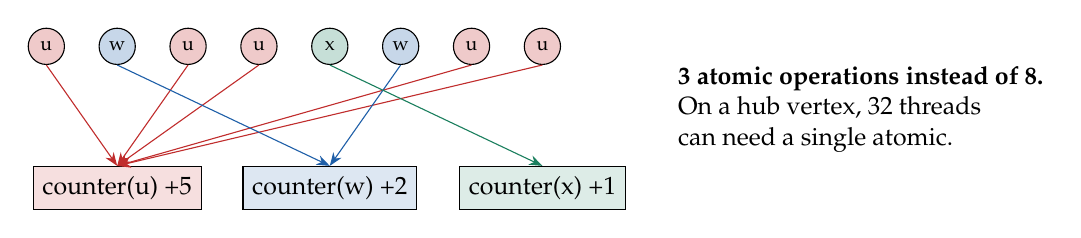
\begin{tikzpicture}[font=\small, >=Stealth, l/.style={draw, circle, minimum size=0.46cm, inner sep=0pt, font=\scriptsize}]
\foreach \i/\c/\v in {0/cHUB/u,1/cGTX/w,2/cHUB/u,3/cHUB/u,4/cGRN/x,5/cGTX/w,6/cHUB/u,7/cHUB/u}
  \node[l, fill=\c!25] (t\i) at (\i*0.9,0.2) {\v};
\node[draw, fill=cHUB!15, minimum height=0.55cm] (cu) at (0.9,-1.6) {counter(u) +5};
\node[draw, fill=cGTX!15, minimum height=0.55cm] (cw) at (3.6,-1.6) {counter(w) +2};
\node[draw, fill=cGRN!15, minimum height=0.55cm] (cx) at (6.3,-1.6) {counter(x) +1};
\foreach \i in {0,2,3,6,7} \draw[->, cHUB] (t\i.south) -- (cu.north);
\foreach \i in {1,5} \draw[->, cGTX] (t\i.south) -- (cw.north);
\draw[->, cGRN] (t4.south) -- (cx.north);
\node[anchor=west, align=left] at (7.9,-0.6) {\textbf{3 atomic operations instead of 8.}\\ On a hub vertex, 32 threads\\ can need a single atomic.};
\end{tikzpicture}
\caption{Warp-cooperative reservation (8 of a warp's 32 threads shown).}
\label{fig:resv}
\end{figure}

\section{Idea 4: Lock-Free Writes, Check Then Swap}
Once it has a slot, a thread links its new version into the edge's chain without taking any lock. To insert or delete
edge $(u,v)$ it:
\begin{enumerate}
\item reads the chain head $h$ for edge $(u,v)$;
\item walks the chain, newest first, looking \emph{only at versions of $v$}: a version written by another transaction
  that is still running, or committed after this transaction started, is a conflict, and the transaction aborts and
  retries later; a version committed before it started is the current state;
\item writes its new version and installs it with a compare-and-swap (CAS): ``make my version the head, but only if the
  head is still $h$'';
\item if the CAS fails, re-checks \emph{only the newly added part}: a version of the same edge means abort; otherwise it
  retries the CAS.
\end{enumerate}

Figure~\ref{fig:cas} shows two threads racing to delete the same edge. Both read the same head and pass the check; only
the first CAS succeeds. The loser's CAS fails because the head has moved, it re-checks the new part, finds the winner's
version of the same edge, and aborts. No lock is ever held, and readers are never blocked.

\begin{figure}[H]
\centering
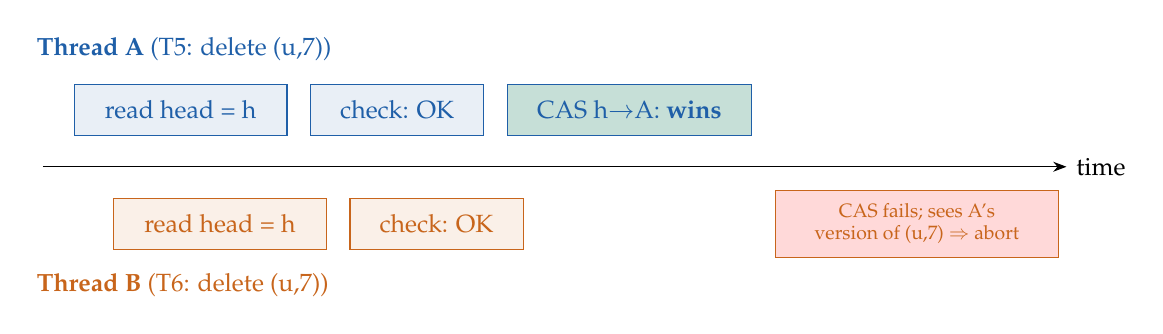
\begin{tikzpicture}[font=\small, >=Stealth]
\draw[->] (0,0) -- (13,0) node[right] {time};
\node[anchor=west, cGTX] at (-0.2,1.5) {\textbf{Thread A} (T5: delete (u,7))};
\node[anchor=west, cORG] at (-0.2,-1.5) {\textbf{Thread B} (T6: delete (u,7))};
\draw[cGTX, fill=cGTX!10] (0.4,0.4) rectangle (3.1,1.05) node[midway] {read head = h};
\draw[cGTX, fill=cGTX!10] (3.4,0.4) rectangle (5.6,1.05) node[midway] {check: OK};
\draw[cGTX, fill=cGRN!25] (5.9,0.4) rectangle (9.0,1.05) node[midway] {CAS h$\to$A: \textbf{wins}};
\draw[cORG, fill=cORG!10] (0.9,-1.05) rectangle (3.6,-0.4) node[midway] {read head = h};
\draw[cORG, fill=cORG!10] (3.9,-1.05) rectangle (6.1,-0.4) node[midway] {check: OK};
\draw[cORG, fill=red!15] (9.3,-1.15) rectangle (12.9,-0.3) node[midway, align=center, font=\scriptsize] {CAS fails; sees A's\\ version of (u,7) $\Rightarrow$ abort};
\end{tikzpicture}
\caption{Check-then-swap: exactly one of two racing writers wins.}
\label{fig:cas}
\end{figure}

\subsection{Per-Edge Rather Than Per-Chain Conflicts}
A chain can hold several edges, because an edge $(u,v)$ is placed on the head at position $\mathrm{hash}(v)$ modulo the
number of heads, and different destinations can collide. Every record stores its destination, so while walking the
chain the writer skips every record that belongs to a different edge; a chain full of other edges' records costs extra
walking steps but never an abort. GTX instead judges conflicts per chain: if the newest record on the chain belongs to
an unfinished transaction, the writer aborts, whichever edge that record is for. Two transactions writing different
edges that share a chain, for example $(u,7)$ and $(u,12)$, then abort each other for no reason (a \emph{false
conflict}). Under our rule, the second writer's first CAS still fails because the shared head moved, but when it
re-checks the new part it finds only a record for destination 7, skips it, retries the CAS and succeeds: both
transactions commit.

\subsection{Why This Is Safe Without a Lock}
\label{sec:safe}
Every write to the same edge must be linked into the \emph{same} head of the current block (same hash, and older blocks
are sealed). Each writer validates from head $h$ and installs with CAS($h \rightarrow$ new), and only one CAS on $h$
can succeed, so the loser always sees the winner's version and aborts: no update is lost. GTX needs a lock because it
checks and installs in separate steps; we combine the two through a CAS on the exact head that was checked. The CAS
cannot suffer from the ABA problem: heads hold slot indices, slots are handed out by a counter that only increases and
are never reused, so a head can never return to an old value. A writer whose head was sealed in the meantime also sees
its CAS fail, because setting the SEAL bit changes the head's value, and retries in the newest block.

\section{Looking Up an Edge and Scanning Neighbours}
Each vertex's blocks are its adjacency list, stored as versions. \emph{Lookup} of $(u,v)$ starts at \code{vcur[u]},
finds the chain head for $v$, and walks that chain newest first, continuing into older blocks if needed; the first
visible version decides (insert: present, delete: absent), usually within one or two memory reads. \emph{Scan} of $u$
visits every slot of every block of $u$ and keeps each insert that is visible to the reader and not deleted before it
started; the 32 threads of a warp scan one vertex together. A traversal such as BFS or DFS is a sequence of scans;
performed inside one read-only transaction, every scan uses the same snapshot, so the traversal sees one consistent
graph while updates continue.

\section{Commit and Visibility}
\label{sec:commit}
Transactions commit in numbered batches (epochs). A warp joins the open batch with a single atomic operation on one
word that holds both the current batch number and the number of writers that joined; each transaction then marks itself
``committed in batch $e$'' and reports done. One special thread, the \emph{advancer}, closes the open batch, waits until
every writer that joined it has reported done, and only then publishes the batch as complete by updating a number
called the \emph{frontier}. A reader takes the frontier as its snapshot and sees exactly the versions of batches up to
it. Because the frontier only moves past a batch when every transaction in it has finished, a reader sees all of a
transaction or none of it, and never waits. An earlier design that re-read the batch number and retried when it changed
livelocked, because the advancer changes that number about once per microsecond; making registration a single atomic
fixed it. The commit machinery costs 9.6--15.5\% of GPU time for single-edge inserts.

The guarantee provided is snapshot isolation: every transaction reads from a snapshot, and two transactions that change
the same edge cannot both commit. Snapshot isolation allows \emph{write skew}: two transactions read the same snapshot
and write \emph{different} edges, breaking a rule that spans both (for example ``every user keeps at least one
contact''). Preventing it requires validating reads at commit (serializability); Section~\ref{sec:ser-proof} covers
the serializable mode added since the mid-term.

\section{Correctness Validation}
GPU concurrency bugs rarely crash; they produce a wrong read once in millions of operations, which a comparison of the
final graph against the list of changes cannot see. Every run therefore records each transaction's snapshot, its commit
batch and the result of every operation, and a checker on the CPU replays the history and verifies that every read and
scan returned what the graph looked like at that transaction's snapshot, that a lookup names the exact version it saw,
that two transactions changing the same edge never overlap, and that the final graph is right. 48 of 48 adversarial
test histories pass. The system was also broken deliberately in three ways (no conflict check, readers ignoring their
snapshot, readers seeing unfinished data); the checker caught all three, two of which pass a simple final-graph test.
Chapter~\ref{ch:proof} extends this validation with a paper proof and a larger test gate.

\section{Differences from GTX}
Table~\ref{tab:diff} summarises what \sys{} keeps from GTX and what it changes.

\begin{table}[H]
\caption{GTX (CPU) versus \sys{}.}
\label{tab:diff}
\small
\begin{singlespace}
\begin{tabular}{@{}P{3.0cm}P{5.6cm}P{6.4cm}@{}}
\toprule
Aspect & GTX (CPU) & \sys{} \\
\midrule
Runs on & CPU, dozens of threads & GPU, thousands of threads in warps of 32 \\
Clash check & per chain: several edges share a chain, so unrelated edges can clash & per edge: only versions of the same edge clash; CAS on the checked head, no lock \\
Full storage & copied into a bigger block & bigger block linked in front, never copied; old chains sealed lazily \\
Getting space & each thread asks on its own & one atomic per warp per vertex \\
Joining a commit batch & group commit & one atomic; one thread publishes finished batches \\
Old versions & cleaned up & compacted between kernel launches (Chapter~\ref{ch:gc}) \\
Supports & vertices, edges, properties & edges on a fixed set of vertices \\
\bottomrule
\end{tabular}
\end{singlespace}
\end{table}

%% ---------------------------------------------------------------------------------------------------- Chapter 5
\chapter{Preliminary Evaluation}
\label{ch:eval}
This chapter describes how the engine was measured and presents three preliminary benchmarks: throughput as
transactions grow, the abort ratio of per-edge versus per-chain conflict detection, and mixed read/write transactions.

\section{Setup and Method}
\begin{itemize}
\item \textbf{Hardware:} NVIDIA RTX~4060 Laptop GPU (8~GB), CUDA~12.8, Windows~11.
\item \textbf{Graph:} $2^{20}$ (about one million) vertices, pre-loaded with 4 million edges.
\item \textbf{Work per run:} about one million operations grouped into transactions of $K$ operations, where $K$ is the
  number of edge operations per transaction ($K=1$: one million single-edge transactions; $K=32$: about 32 thousand
  transactions of 32 operations).
\item \textbf{Workloads:} \emph{uniform} (edges between random vertices, few collisions); \emph{50\% hub} (half of all
  operations touch one single vertex, a worst case for collisions); \emph{Zipf} (realistic skew: a few very popular
  vertices, many unpopular ones).
\item \textbf{Input:} a seeded generator produces an identical stream of operations for every configuration.
\item \textbf{Timing:} GPU time of the transaction kernel, measured with CUDA events; loading the initial edges is
  excluded.
\item \textbf{Repetitions:} one warm-up run followed by five measured runs; the median is reported.
\item \textbf{Metrics:} \emph{effective} edge changes per second count only operations that actually changed the graph
  (inserting an edge that already exists, or a read, changes nothing); the \emph{abort ratio} is the fraction of
  attempts that hit a conflict and had to retry.
\end{itemize}

\textbf{GTX rules.} To isolate the effect of our design, we compare against our own engine run with GTX's original
behaviour: per-chain conflict detection and per-thread slot reservation. Everything else (GPU, code, data structure,
workload) is identical, so any difference comes only from the design changes. This configuration shows what a direct
port of GTX to the GPU would do; it is not the CPU GTX system itself.

\section{Throughput as Transactions Grow}
Figure~\ref{fig:ksweep} and Table~\ref{tab:ksweep} show effective edge inserts per second as $K$ grows from 1 to 32.
Our engine stays at 140--180 million per second on uniform graphs and above 120 million up to $K=8$ even when half of
all operations hit one vertex. GTX rules drops sharply at $K=32$ (78.5 million on uniform). On the hub, even our engine
drops at $K=32$, because 32-edge transactions that all touch the same vertex genuinely conflict. The hub lines are lower
overall because many hub inserts try to add an edge that already exists and are not counted as effective.

\begin{figure}[H]
\centering
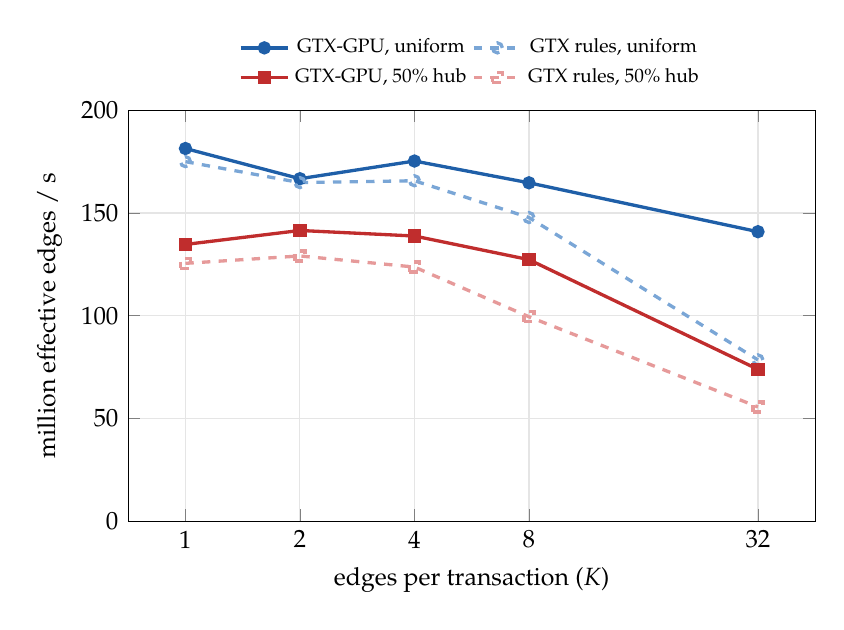
\begin{tikzpicture}
\begin{axis}[width=0.85\textwidth, height=6.8cm,
  xmode=log, log basis x=2, xtick={1,2,4,8,32}, xticklabels={1,2,4,8,32},
  ymin=0, ymax=200, grid=major, grid style={black!10},
  xlabel={edges per transaction ($K$)}, ylabel={million effective edges / s},
  tick label style={font=\small}, label style={font=\small},
  legend style={font=\scriptsize, at={(0.5,1.03)}, anchor=south, legend columns=2, draw=none}]
\addplot[cGTX, very thick, mark=*, mark size=1.8pt] coordinates {(1,181.4)(2,166.7)(4,175.3)(8,164.7)(32,140.9)};
\addlegendentry{\sys{}, uniform}
\addplot[cCONS, very thick, dashed, mark=o, mark size=1.8pt] coordinates {(1,175.0)(2,164.8)(4,165.7)(8,147.8)(32,78.5)};
\addlegendentry{GTX rules, uniform}
\addplot[cHUB, very thick, mark=square*, mark size=1.8pt] coordinates {(1,134.7)(2,141.5)(4,138.8)(8,127.3)(32,73.9)};
\addlegendentry{\sys{}, 50\% hub}
\addplot[cHUBL, very thick, dashed, mark=square, mark size=1.8pt] coordinates {(1,125.5)(2,129.1)(4,123.7)(8,99.5)(32,55.6)};
\addlegendentry{GTX rules, 50\% hub}
\end{axis}
\end{tikzpicture}
\caption{Effective edge inserts per second versus transaction size.}
\label{fig:ksweep}
\end{figure}

\begin{table}[H]
\caption{Million effective edge inserts per second.}
\label{tab:ksweep}
\small
\begin{singlespace}
\centering
\begin{tabular}{@{}lrrrrr@{}}
\toprule
$K$ & 1 & 2 & 4 & 8 & 32 \\
\midrule
Uniform, \sys{} & 181.4 & 166.7 & 175.3 & 164.7 & 140.9 \\
Uniform, GTX rules & 175.0 & 164.8 & 165.7 & 147.8 & 78.5 \\
50\% hub, \sys{} & 134.7 & 141.5 & 138.8 & 127.3 & 73.9 \\
50\% hub, GTX rules & 125.5 & 129.1 & 123.7 & 99.5 & 55.6 \\
\bottomrule
\end{tabular}
\end{singlespace}
\end{table}

\section{Abort Ratio: Per-Edge Versus Per-Chain Conflicts}
Figure~\ref{fig:aborts} shows the fraction of attempts that abort. With GTX's per-chain rule, transactions that touch
different edges still abort each other when those edges share a chain, and the larger the transaction, the more likely
this is: at $K=32$ almost half of all attempts are thrown away (45.4\% uniform, 42.5\% hub). Checking conflicts per
edge removes all of these false aborts on uniform graphs (0\%); on the hub, the remaining 25.9\% are true conflicts on
the same edges, which no correct rule can avoid. The result is a throughput gain of 1.11$\times$ (uniform, $K=8$),
1.80$\times$ (uniform, $K=32$), 1.28$\times$ (hub, $K=8$) and 1.33$\times$ (hub, $K=32$) over GTX rules.

\begin{figure}[H]
\centering
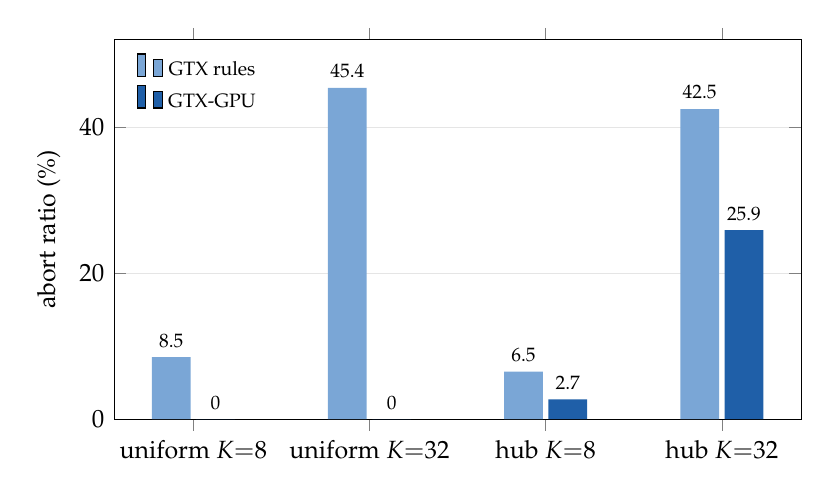
\begin{tikzpicture}
\begin{axis}[width=0.85\textwidth, height=6.4cm, ybar, bar width=14pt,
  ymin=0, ymax=52, symbolic x coords={u8,u32,h8,h32}, xtick=data,
  xticklabels={{uniform $K{=}8$},{uniform $K{=}32$},{hub $K{=}8$},{hub $K{=}32$}},
  tick label style={font=\small}, ylabel={abort ratio (\%)}, label style={font=\small},
  ymajorgrids, grid style={black!10}, enlarge x limits=0.15,
  nodes near coords, nodes near coords style={font=\scriptsize},
  legend style={font=\scriptsize, at={(0.02,0.98)}, anchor=north west, draw=none}]
\addplot[fill=cCONS, draw=none] coordinates {(u8,8.5) (u32,45.4) (h8,6.5) (h32,42.5)};
\addlegendentry{GTX rules}
\addplot[fill=cGTX, draw=none] coordinates {(u8,0) (u32,0) (h8,2.7) (h32,25.9)};
\addlegendentry{\sys{}}
\end{axis}
\end{tikzpicture}
\caption{Abort ratio (wasted attempts) at $K=8$ and $K=32$.}
\label{fig:aborts}
\end{figure}

\section{Mixed Read/Write Transactions}
Figure~\ref{fig:mix} and Table~\ref{tab:mix} show transactions of $K=4$ operations with 40\% inserts, 30\% deletes and
30\% point reads. The engine commits 50.9 million transactions per second on uniform graphs and 50.5 million on the
50\% hub workload, and 34.8 million on a Zipf graph; fewer than 2\% of attempts abort in every case. On pure
insert/delete churn with single-edge transactions it sustains 156 million (uniform) and 144 million (R-MAT) edge
changes per second.

\begin{figure}[H]
\centering
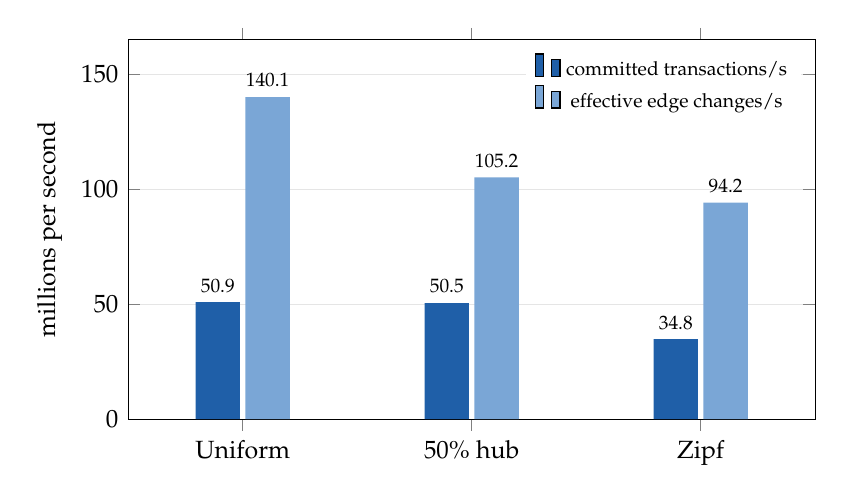
\begin{tikzpicture}
\begin{axis}[width=0.85\textwidth, height=6.4cm, ybar, bar width=16pt,
  ymin=0, ymax=165, symbolic x coords={U,H,Z}, xtick=data,
  xticklabels={Uniform, 50\% hub, Zipf}, tick label style={font=\small},
  ylabel={millions per second}, label style={font=\small},
  ymajorgrids, grid style={black!10}, enlarge x limits=0.25,
  nodes near coords, nodes near coords style={font=\scriptsize},
  legend style={font=\scriptsize, at={(0.98,0.98)}, anchor=north east, draw=none}]
\addplot[fill=cGTX, draw=none] coordinates {(U,50.9) (H,50.5) (Z,34.8)};
\addlegendentry{committed transactions/s}
\addplot[fill=cCONS, draw=none] coordinates {(U,140.1) (H,105.2) (Z,94.2)};
\addlegendentry{effective edge changes/s}
\end{axis}
\end{tikzpicture}
\caption{Throughput on mixed read/write transactions ($K=4$).}
\label{fig:mix}
\end{figure}

\begin{table}[H]
\caption{Mixed read/write transactions ($K=4$).}
\label{tab:mix}
\small
\begin{singlespace}
\centering
\begin{tabular}{@{}lrrr@{}}
\toprule
Workload & Transactions/s & Effective edges/s & Abort ratio \\
\midrule
Uniform & 50.9 M & 140.1 M & 1.1\% \\
50\% hub & 50.5 M & 105.2 M & 1.9\% \\
Zipf & 34.8 M & 94.2 M & 1.1\% \\
\bottomrule
\end{tabular}
\end{singlespace}
\end{table}

%% ---------------------------------------------------------------------------------------------------- Chapter 6
\addtocontents{toc}{\protect\enlargethispage{2\baselineskip}}
\chapter{Extended Evaluation}
\label{ch:exteval}
This chapter extends the preliminary evaluation of Chapter~\ref{ch:eval}: it compares \sys{} with lock-based,
STM-based, non-transactional and batch-update baselines on the same streams, adds concurrent snapshot readers,
serializable transactions and real graphs, and lists the cases in which \sys{} is slower.

\section{Setup}
\label{sec:extsetup}
\begin{itemize}
\item \textbf{Hardware and graph:} as in Chapter~\ref{ch:eval}: RTX~4060 Laptop GPU, $2^{20}$ vertices, 4 million
  initial edges and about one million operations per run (or $2^{18}$ transactions of $K=4$ operations).
\item \textbf{New workloads:} \emph{churn} (50\% inserts, 50\% deletes); \emph{R-MAT} (a synthetic power-law
  generator); \emph{identical-edge contention} (half of all operations target a small set of 64 or 1,024 hot edges);
  and \emph{readers} (50\% or 90\% of transactions are read-only, and 10\% of their operations are adjacency scans).
\item \textbf{Repetitions:} one warm-up and five measured runs per system and scenario, each in its own process. The
  speedup is the ratio of median committed transactions per second, with a 95\% bootstrap confidence interval. A run
  that does not finish within 90~s is recorded as DNF; its speedup is then a lower bound (written ``$>$'').
\item \textbf{Two campaigns.} The numbers of this chapter come from a second measurement campaign (November 2026),
  run with the final binaries in one session. Every kernel ran 1.4--2.7$\times$ faster than in the September
  campaign of Chapter~\ref{ch:eval}. The September source code rebuilt with the November compiler times identically,
  so the shift is not caused by the code; its system-side cause (driver, power state) was not isolated. Absolute
  numbers from the two campaigns are therefore never compared with each other; every ratio below is taken within the
  November campaign.
\end{itemize}

\textbf{Baselines.} All transactional baselines share one storage layout: a per-vertex hash table of neighbours plus a
per-vertex degree counter, \emph{pre-sized} from the whole workload, so unlike \sys{} they never pay for growth.
\begin{itemize}
\item \textbf{2PL}: strict two-phase locking with per-vertex reader-writer spinlocks, acquired in sorted vertex order
  (deadlock-free).
\item \textbf{TL2 STM}: a word-based software transactional memory in the style of TL2~\cite{tl2} (global version clock,
  versioned locks, buffered writes, read-set validation at commit).
\item \textbf{TL2 STM without degree word}: the same STM without the per-vertex degree counter. It avoids the hub hot
  spot described in Chapter~\ref{ch:lit}, but it cannot answer degree queries transactionally.
\item \textbf{Non-transactional CAS}: lock-free updates with compare-and-swap and no transactions at all. It gives no
  atomicity and no snapshots, and serves only as a lower bound on the cost of synchronisation.
\item \textbf{GPMA+}~\cite{gpma}: the authors' batch-update implementation (the upstream code and a Windows port, within
  2\% of each other).
\end{itemize}
The timed runs are not checked (checking would dominate their time); separate checked runs of every system validate
the results with the history checker (Section~\ref{sec:checkerext}). Reader scenarios use each baseline's faster scan
mode (per-thread or warp-cooperative).

\section{Headline Comparison}
\label{sec:headline}
Table~\ref{tab:headline} gives \sys{}'s speedup over each baseline. Where synchronisation is hard (hubs, power-law
skew, large transactions, readers) \sys{} is one to four orders of magnitude faster than 2PL and TL2: on power-law
churn 2PL serialises on hub locks (463$\times$ on R-MAT; it does not finish on Zipf), and TL2 is 96--706$\times$
slower. On uniform graphs with small transactions the situation reverses (Section~\ref{sec:losses}).
Figure~\ref{fig:headline} shows the speedup over TL2 on a logarithmic scale.

\begin{table}[H]
\caption{Speedup of \sys{} in committed transactions per second ($>1$: \sys{} faster). ``$>$'': the baseline did not
finish within 90~s.}
\label{tab:headline}
\small
\begin{singlespace}
\begin{tabular}{@{}P{6.9cm}rrrr@{}}
\toprule
Scenario & 2PL & TL2 STM & \makecell{TL2 STM\\no degree} & \makecell{CAS\\(no txn)} \\
\midrule
R-MAT, 90\% snapshot readers & \textbf{19.9} & \textbf{20.6} & \textbf{14.2} & 0.41 \\
Zipf, 50\% readers & \textbf{$>$616} & \textbf{27.9} & \textbf{7.4} & 0.53 \\
Serializable read-write, Zipf ($K{=}4$) & \textbf{2,128} & \textbf{420} & 0.64 & -- \\
Serializable read-write, 50\% hub & \textbf{$>$26,903} & \textbf{652} & 0.75 & -- \\
R-MAT churn, $K{=}4$ & \textbf{463} & \textbf{96} & 0.72 & 0.31 \\
Zipf churn, $K{=}4$ & \textbf{$>$21,863} & \textbf{706} & 0.73 & 0.37 \\
Identical-edge contention, 1,024 hot edges & \textbf{4.0} & \textbf{9.8} & \textbf{6.4} & 0.17 \\
Identical-edge contention, 64 hot edges & \textbf{6.2} & \textbf{5.9} & \textbf{5.6} & 0.07 \\
Large transactions, $K{=}32$, uniform & 1.06 & \textbf{85} & \textbf{8.1} & 0.33 \\
Large transactions, $K{=}32$, 50\% hub & \textbf{$>$18,934} & \textbf{7,444} & \textbf{3.2} & 0.29 \\
50\% hub inserts, $K{=}8$ & \textbf{$>$28,675} & \textbf{795} & 1.01 & 0.44 \\
Uniform inserts, $K{=}1$ & 0.56 & 0.97 & 0.62 & 0.47 \\
Uniform churn, $K{=}4$ & 0.44 & 1.67 & 0.70 & 0.33 \\
Serializable read-write, uniform & 0.49 & 1.61 & 0.80 & -- \\
Uniform, 50\% readers & 0.55 & 1.32 & 0.77 & 0.38 \\
\bottomrule
\end{tabular}
\end{singlespace}
\end{table}

\begin{figure}[H]
\centering
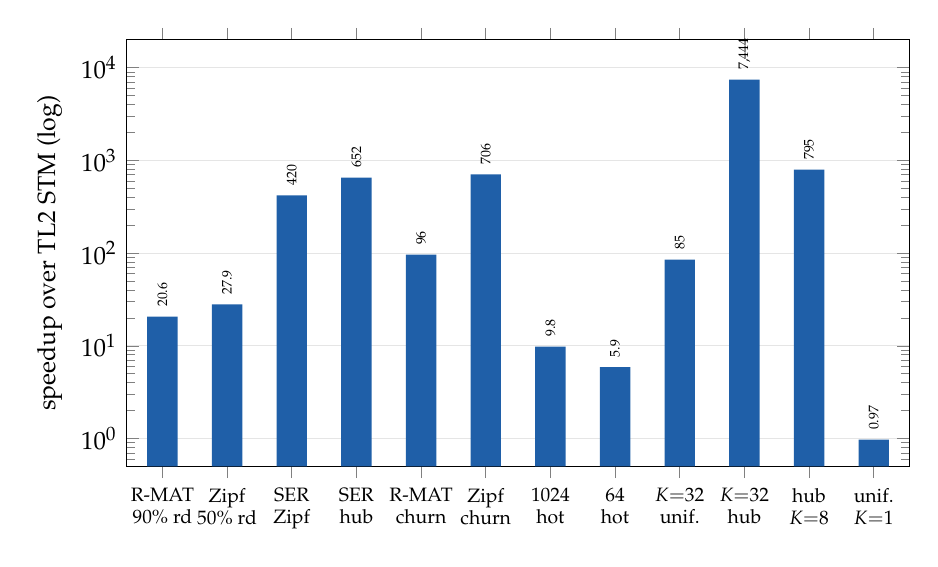
\begin{tikzpicture}
\begin{axis}[width=0.95\textwidth, height=7cm, ybar, bar width=11pt, ymode=log, log origin=infty,
  ymin=0.5, ymax=20000, symbolic x coords={a,b,c,d,e,f,g,h,i,j,k,l},
  xtick=data, xticklabels={{R-MAT\\90\% rd}, {Zipf\\50\% rd}, {SER\\Zipf}, {SER\\hub}, {R-MAT\\churn},
  {Zipf\\churn}, {1024\\hot}, {64\\hot}, {$K{=}32$\\unif.}, {$K{=}32$\\hub}, {hub\\$K{=}8$}, {unif.\\$K{=}1$}},
  xticklabel style={align=center, font=\scriptsize}, tick label style={font=\small},
  ylabel={speedup over TL2 STM (log)}, label style={font=\small},
  ymajorgrids, grid style={black!10}, enlarge x limits=0.05,
  nodes near coords={\pgfmathprintnumber[fixed, precision=2]{\pgfplotspointmeta}},
  point meta=rawy, nodes near coords style={font=\tiny, rotate=90, anchor=west}]
\addplot[fill=cGTX, draw=none] coordinates {(a,20.6) (b,27.9) (c,420) (d,652) (e,96) (f,706) (g,9.8) (h,5.9)
  (i,85) (j,7444) (k,795) (l,0.97)};
\end{axis}
\end{tikzpicture}
\caption{Speedup of \sys{} over the TL2 STM (November campaign).}
\label{fig:headline}
\end{figure}

\section{Concurrent Snapshot Readers}
\label{sec:readers}
Readers are where versions pay off most. With 90\% read-only transactions on R-MAT, \sys{}'s readers never block
writers, never abort and never wait. \sys{} commits 43.9 million transactions per second with an overall abort ratio
of 0.02\%, against 87\% for TL2, and is 19.9$\times$, 20.6$\times$ and 14.2$\times$ faster than 2PL, TL2 and TL2 without
degree word. The 99th-percentile latency of a read-only transaction is 0.69--0.74~ms for \sys{} against 24--122~ms for
the transactional baselines. Under Zipf with 50\% readers, 2PL does not finish, and \sys{} is 27.9$\times$ faster than
TL2. Warp-cooperative scanning is essential: with one thread per scan, \sys{} was 5.9$\times$ slower on Zipf readers
(September campaign), because a scan reads every 32-byte version, including aborted ones.

\section{Serializable Transactions}
In its serializable mode \sys{} additionally checks at commit that nothing the transaction read has changed since its
snapshot (Section~\ref{sec:ser-proof}); this costs 6--15\% relative to snapshot isolation. With read-write transactions of $K=4$ operations (20\% of them read-only), serializable \sys{} is 2,128$\times$ and
420$\times$ faster than 2PL and TL2 on Zipf, and 652$\times$ faster than TL2 on the 50\% hub workload, where 2PL does
not finish. TL2 without degree word is faster in these write-dominated mixes: \sys{} reaches 0.64$\times$ (Zipf),
0.75$\times$ (hub) and 0.80$\times$ (uniform) of it. All systems pass the serializability check in these runs.

\section{Real Graphs}
\label{sec:snap}
Four graphs from the SNAP collection~\cite{snap} are replayed as sliding-window streams: the edges are shuffled with a
fixed seed, the first 80\% form the initial graph, inserts take unseen edges from the rest, and deletes remove the
oldest initial edges. Table~\ref{tab:snap} shows the result. wiki-Talk, which has a vertex of degree 100,022, behaves
like the synthetic hub workloads: \sys{} wins by one to three orders of magnitude. Graphs without large hubs
(roadNet-CA, cit-Patents) behave like the uniform workloads: on their update streams \sys{} is 0.66--0.84$\times$
of 2PL. \sys{} is faster than
GPMA+ on every real stream.

\begin{table}[H]
\caption{Speedup of \sys{} on real graphs (churn: 50\% inserts and 50\% deletes; GPMA+ in effective edge changes per
second).}
\label{tab:snap}
\small
\begin{singlespace}
\begin{tabular}{@{}P{4.4cm}P{3.0cm}rrr@{}}
\toprule
Graph ($|V|$, $|E|$, max.\ degree) & Stream & 2PL & TL2 STM & GPMA+ \\
\midrule
wiki-Talk (2.39M, 5.0M, 100,022) & inserts, $K{=}1$ & \textbf{34} & \textbf{96} & \textbf{51.5} \\
 & churn, $K{=}4$ & \textbf{1,103} & \textbf{395} & -- \\
 & 90\% readers, $K{=}4$ & \textbf{196} & \textbf{30} & -- \\
soc-pokec (1.63M, 30.6M, 8,763) & inserts, $K{=}1$ & 1.01 & \textbf{1.81} & \textbf{15.2} \\
 & readers, $K{=}4$ & \textbf{1.19} & \textbf{6.80} & -- \\
cit-Patents (3.77M, 16.5M, 770) & inserts, $K{=}1$ & 0.75 & 1.08 & \textbf{12.3} \\
 & readers, $K{=}4$ & 1.12 & \textbf{2.41} & -- \\
roadNet-CA (1.97M, 5.5M, 12) & inserts, $K{=}1$ & 0.77 & 1.06 & \textbf{296} \\
 & readers, $K{=}4$ & 0.84 & 1.38 & -- \\
\bottomrule
\end{tabular}
\end{singlespace}
\end{table}

\section{Batch Size Against GPMA+}
GPMA+ applies updates in batches and makes each batch atomic as a whole. For a fair comparison, \sys{} is run as one
kernel launch per batch, with its snapshot published between launches. Table~\ref{tab:batch} shows the total GPU time
for 4 million uniform churn operations. \sys{} is 1.8--16.5$\times$ faster at every batch size; its time is flat from
$2^{16}$ operations per batch, while GPMA+ amortises its sorting and rebalancing only at very large batches. GPMA+ also
loses the order of operations inside a batch: when a batch inserts and deletes the same edge, its final graph is wrong
(86 wrong edges at $2^{10}$, rising to 360,800 at $2^{22}$).

\begin{table}[H]
\caption{Batch-size sweep, uniform churn, 4M operations, total GPU time in ms.}
\label{tab:batch}
\small
\begin{singlespace}
\centering
\begin{tabular}{@{}lrrrrrrr@{}}
\toprule
Batch size & $2^{10}$ & $2^{12}$ & $2^{14}$ & $2^{16}$ & $2^{18}$ & $2^{20}$ & $2^{22}$ \\
\midrule
\sys{} & 224.9 & 59.5 & 27.9 & 20.9 & 19.0 & 18.5 & 18.4 \\
GPMA+ (faster version) & 3,198.7 & 978.9 & 292.5 & 123.9 & 99.0 & 77.1 & 33.4 \\
Speedup of \sys{} & 14.2 & 16.5 & 10.5 & 5.9 & 5.2 & 4.2 & 1.8 \\
\bottomrule
\end{tabular}
\end{singlespace}
\end{table}

\section{Where \sys{} Is Slower}
\label{sec:losses}
Table~\ref{tab:losses} lists every scenario in which \sys{} loses. The gap to 2PL on uniform graphs is not caused by
the write path: removing the whole versioned install (which is not a valid execution) still leaves \sys{} 16--21\%
behind 2PL on uniform inserts. The transaction machinery alone (status words, batches, the retry loop and the advancer)
costs more than 2PL's whole run when there is no contention.

\begin{table}[H]
\caption{Scenarios in which \sys{} is slower (\sys{} / baseline throughput).}
\label{tab:losses}
\small
\begin{singlespace}
\begin{tabular}{@{}P{5.0cm}P{1.8cm}P{8.0cm}@{}}
\toprule
Scenario & Ratio & Reason \\
\midrule
uniform, small transactions, vs 2PL & 0.37--0.56 & transaction machinery; uncontended locks are cheap \\
real graphs without hubs, vs 2PL & 0.66--0.84 & same cause (roadNet-CA, cit-Patents) \\
write-heavy work vs TL2 without degree word & 0.58--0.87 & that STM cannot answer degree queries, and is 5.4--20.6$\times$ slower once scanning readers arrive \\
almost any scenario vs non-transactional CAS & 0.07--0.71 & CAS offers no atomicity and no snapshots \\
memory vs pre-sized hash tables & 3--19$\times$ & versions, chain heads and block layout (Chapter~\ref{ch:gc}) \\
long update streams with compaction & 0.70--0.81 & compaction pauses (Chapter~\ref{ch:gc}) \\
\bottomrule
\end{tabular}
\end{singlespace}
\end{table}

%% ---------------------------------------------------------------------------------------------------- Chapter 7
\chapter{Garbage Collection of Old Versions}
\label{ch:gc}
This chapter addresses the memory problem left open in the mid-term report.

\section{The Problem}
\sys{} allocates versions, chain heads and blocks from one pre-allocated GPU arena by moving a pointer forward, and
never reuses them. This is what makes lock-free writes safe (Section~\ref{sec:safe}), but any long stream of updates
eventually exhausts the arena: without reclamation \sys{} runs out of a 20-million-slot arena within 1--13 rounds of
$2^{18}$ transactions. Memory was measured before any redesign, and most of it is \emph{layout}, not garbage: unused
capacity in each vertex's newest block (8$\times$ growth) is 43--61\% of all bytes, while reclaimable garbage (aborted,
overwritten and deleted versions) is only 0\% on uniform inserts, 4\% on Zipf churn and 9--14\% with hot edges.
Garbage is a small share of memory at any moment, but it is the only part that grows without bound. A first design,
merging old blocks while kernels ran, was proven correct but fell to 0.33$\times$ throughput; it remains in the code,
switched off.

\section{Implementation: Quiescent Compaction}
\label{sec:qc}
The working design reclaims memory \emph{between} kernel launches. At that moment no transaction is running and no
snapshot is open, so nothing can still be reading an old version, and reclamation needs no locks or announcements:
the lock-free hot path is unchanged. Compaction (Figure~\ref{fig:qc}):
\begin{enumerate}
\item is triggered only when the arena could not absorb 1.5$\times$ the largest growth of any previous round;
\item computes the graph visible at the latest published snapshot (the frontier $F$);
\item discards the whole version store and rebuilds it as if that graph had just been loaded: one block per vertex,
  sized to its live edges plus slack, every edge stored as one committed insert of a single ``loader'' transaction;
\item rebuilds large vertices (more than 4,096 slots, in chunks of 512) with a whole thread block and small ones with
  one warp, which cut the pause on Zipf from 27.4 to 10.0~ms.
\end{enumerate}

\begin{figure}[H]
\centering
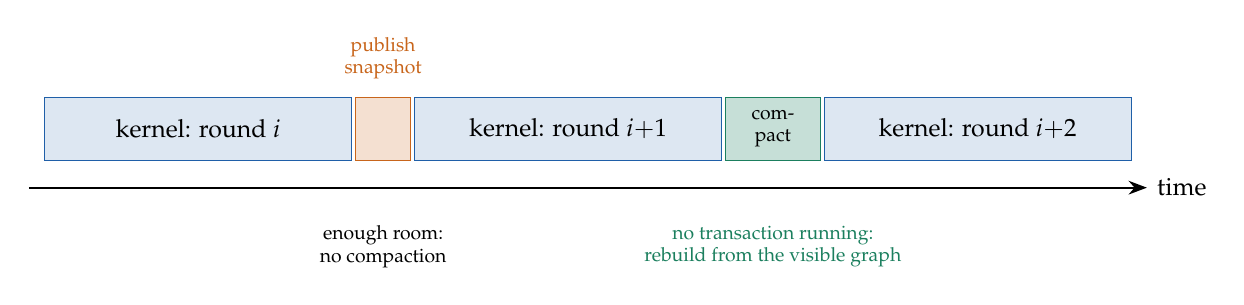
\begin{tikzpicture}[font=\small, >=Stealth]
\draw[->, thick] (0,0) -- (14.2,0) node[right] {time};
\foreach \x/\l in {0.2/round $i$, 4.9/round $i{+}1$, 10.1/round $i{+}2$} {
  \draw[fill=cGTX!15, draw=cGTX] (\x,0.35) rectangle (\x+3.9,1.15) node[midway] {kernel: \l};
}
\draw[fill=cORG!20, draw=cORG] (4.15,0.35) rectangle (4.85,1.15);
\node[cORG, font=\scriptsize, align=center] at (4.5,1.65) {publish\\snapshot};
\draw[fill=cGRN!25, draw=cGRN] (8.85,0.35) rectangle (10.05,1.15) node[midway, font=\scriptsize, align=center] {com-\\pact};
\node[cGRN, align=center, font=\scriptsize] at (9.45,-0.75) {no transaction running:\\rebuild from the visible graph};
\node[align=center, font=\scriptsize] at (4.5,-0.75) {enough room:\\no compaction};
\end{tikzpicture}
\caption{Quiescent compaction runs only between kernel launches, and only when the next round might not fit.}
\label{fig:qc}
\end{figure}

\paragraph{Outcome.} Pass criteria were written before the code: (Q1) no out-of-memory and flat memory, (Q2)
throughput, (Q3) correctness tests with deliberately broken versions, (Q4) reported pauses. On 64 rounds of $2^{18}$
transactions (67 million effective writes against a 20-million-slot arena), \sys{} with compaction completes every
round on uniform and Zipf churn, where it otherwise fails within 1--7 rounds, and its memory stays flat (last/middle
third 0.999--1.001). It reaches 0.70--0.81$\times$ the throughput of \sys{} given a 3$\times$ larger arena, with pauses
of 8--12~ms at the median (at most 21~ms). Memory is bounded by the size of the live graph, not by a constant: with
1,024 hot edges the live graph itself grows from 4.0M to 10.3M edges, and a 40M arena is needed to complete 64 rounds.

%% ---------------------------------------------------------------------------------------------------- Chapter 8
\chapter{Correctness Proof}
\label{ch:proof}
GPU concurrency bugs are silent: a missing memory-ordering edge produces a wrong read once in millions of operations,
or never on one particular GPU. The history checker of Chapter~\ref{ch:framework} validates the histories that
actually occurred, but cannot see a bug that never manifests. This chapter summarises a paper proof that every history
of \sys{} satisfies snapshot isolation (and serializability in the serializable mode), and the extended tests that
exercise each step of it. The proof is written by hand against the GPU memory model; it is not machine-checked. The
full proof, with every lemma mapped to the code line it depends on and the test that exercises it, is in
\code{design/proof.md}.

\section{Model and Assumptions}
\label{sec:proof-model}
The proof reasons about the PTX memory model of NVIDIA GPUs: \emph{happens-before} is built from release/acquire
operations, fences and the order of atomic operations on each memory word. It assumes:
\begin{enumerate}[label=\textbf{A\arabic*}]
\item \textbf{No reuse.} Version slots, chain heads, blocks and transaction ids are never reused (the arena is only
  extended).
\item \textbf{Memory model.} All protocol atomics are device-scope. Ordering between the threads of a warp comes only
  from \code{\_\_syncwarp} and fences, never from warp vote or shuffle instructions, which the CUDA guide states imply
  no memory ordering.
\item \textbf{No overflow.} Batch numbers fit in 32 bits, and the arena has fewer than $2^{31}$ slots.
\item \textbf{Quiescent boundaries.} Snapshots are published and compaction runs only between kernel launches.
\end{enumerate}
Notation: for a transaction $T$, $rts(T)$ is the snapshot (frontier) it read and $e(T)$ its commit batch. $S(r)$ is
the graph obtained by applying, in batch order, the writes of every transaction committed in a batch $\le r$.

\section{Status Words and Commit Batches}
Five lemmas establish that the commit machinery of Section~\ref{sec:commit} behaves as intended:
\begin{itemize}
\item \textbf{L1 (status finality).} Each attempt writes its status word at most once, with a final value
  (committed in batch $e$, or aborted); every read returns 0 or that value.
\item \textbf{L2 (exact registration).} The advancer closes a batch with one atomic exchange on the word that writers
  join with \code{fetch\_add}; exactly the writers that joined before the exchange belong to that batch.
\item \textbf{L3 (frontier safety).} If a reader sees frontier $r$, then every transaction committed in a batch $\le r$
  has written its final status, and all its versions, before that read (a release/acquire chain through the advancer).
\item \textbf{L4 (fresh batches).} Every writer commits in a batch strictly later than its snapshot: $e(T) > rts(T)$.
\item \textbf{L5 (stable visibility).} For a reader with snapshot $r$, a version is visible exactly when its writer is
  the reader itself or committed in a batch $\le r$, every time the reader looks at it.
\end{itemize}

\section{Write--Write Exclusion}
\begin{itemize}
\item \textbf{L6 (one chain per edge per block; sealing).} Within a block, all versions of an edge go to one chain head.
  A writer that moves to a newer block first seals the old head, after which no compare-and-swap can link into it.
\item \textbf{L7 (validate, then swap on the observed head).} A writer that links its version with a compare-and-swap
  on head value $h$ has walked every version reachable from $h$; after a failed swap it re-walks the new prefix first.
\end{itemize}

\begin{quote}
\textbf{Theorem 1 (version order).} The committed versions of an edge are totally ordered, and for consecutive
versions by $T_1$ then $T_2$: $e(T_1) \le rts(T_2) < e(T_2)$.
\end{quote}
\emph{Sketch.} Take two committed versions of one edge, the second linked later. If they are in the same block, the
second writer walked the first (L7). If the first is in an older block, the second writer sealed its head and walked
it (L6). The reverse case is impossible. The second writer did not abort, so the version it found was visible to it
(L5), hence committed at or before its snapshot, and its own batch is later (L4). This is first-committer-wins: no two
transactions that overlap in time both commit a write to the same edge. \hfill$\square$

\section{Reads and Scans}
\begin{quote}
\textbf{Theorem 2 (point reads).} A lookup of edge $(u,v)$ by a transaction with snapshot $r$ returns $S(r)$ for that
edge, overlaid with the transaction's own earlier writes.

\textbf{Theorem 3 (scans).} A scan of $u$ returns exactly the neighbours of $u$ in $S(r)$, overlaid with the
transaction's own writes.
\end{quote}
\emph{Sketch.} A lookup returns the first own or visible version on the chain; by Theorem 1 that is the version with
the largest batch $\le r$. Two further lemmas cover scans. \textbf{L8 (block reachability):} every block that holds a
visible version is reachable from the vertex's current-block pointer, and the slot count a reader sees covers it; this
needs the slot reservation to be an acquire-release operation, and the version with a relaxed reservation is exactly a
defect our checker had found earlier. \textbf{L9 (invalidation word):} the \code{its} field of an insert is written
only by the transaction that deleted it, so a scan counts an insert exactly when it is the newest visible version of
its edge. \hfill$\square$

\begin{quote}
\textbf{Theorem 4 (snapshot isolation).} Every committed transaction reads $S(rts)$ overlaid with its own writes; its
writes become visible to other snapshots all at once; and no two concurrent committed transactions write the same
edge.
\end{quote}
This follows from Theorems 1--3 and L5: visibility depends only on one status word or batch number per transaction,
and snapshots cover only completed batches, so no reader sees a transaction half done.

\section{Serializability}
\label{sec:ser-proof}
In the serializable mode a writer validates at commit that every edge it read and every vertex it scanned is unchanged
since its snapshot. It joins its commit batch \emph{before} validating, as in Silo~\cite{silo}; read-only transactions
need no validation.
\textbf{L10} shows that if $T$ read a version that a committed $U$ later overwrote, then $T$ joined its batch strictly
before $U$; otherwise $T$'s validation would have seen $U$'s version and aborted.
\begin{quote}
\textbf{Theorem 5 (serializability).} Order writers by (batch, position of their join operation) and
read-only transactions at the end of their snapshot batch. Every write--write, write--read and read--write dependency
respects this order, so the serialization graph has no cycle and the history is serializable.
\end{quote}

\section{Garbage Collection}
The merging design of Chapter~\ref{ch:gc} is covered by four further lemmas (L11--L14: which versions may be dropped,
consistent forwarding to the merged block, validation under copies, and safe reuse through announcements). For
compaction, assumption A1 is weakened to ``no reuse \emph{within} one kernel run'':
\begin{itemize}
\item \textbf{L15 (quiescent state).} When compaction runs, no transaction is in flight, every committed transaction
  is in a batch $\le F$, and all memory written by the previous kernel is visible.
\item \textbf{L16 (live set).} The compaction kernels collect exactly the edges that a snapshot at $F$ would see, each
  once.
\item \textbf{L17 (rebuild).} The rebuilt store equals what the initial loader would produce for that edge set.
\end{itemize}
\begin{quote}
\textbf{Theorem 6 (correctness across compactions).} A long run of kernel launches, some separated by compactions,
satisfies snapshot isolation (serializability in the serializable mode) as a whole.
\end{quote}
\emph{Sketch.} Within each run Theorems 1--5 hold from that run's start state. A compacting boundary replaces the store
by an equivalent freshly loaded one (L15--L17), and no transaction spans two runs, so placing all of run $k$ before run
$k{+}1$ is consistent with every run's order and with real time. \hfill$\square$

\section{Defects Found by the Proof}
Writing the proof found two ordering gaps that no test had ever observed:
\begin{itemize}
\item \textbf{D11:} commit registration ordered the threads of a warp only through warp vote and shuffle instructions,
  which carry no memory ordering (needed by L4 and L10);
\item \textbf{D12:} in warp-cooperative scans every thread loaded the block list itself, although only one thread had
  synchronised with the frontier.
\end{itemize}
Both are fixed (a \code{\_\_syncwarp} around registration; the synchronised thread reads the block list and broadcasts
it), at a cost of at most 1\%.

\section{Testing the Proof}
\label{sec:proof-tests}
\label{sec:checkerext}
\textbf{Correctness gate.} The 48 adversarial histories of the mid-term grew into a gate of nine sections
(Table~\ref{tab:gate}) with \textbf{219 cases and 0 unexpected results}. A history passes only if every read, scan and
write agrees with the snapshot rule, no two committed writers of an edge overlap, the final graph is right, and, in the
serializable mode, the serialization graph has no cycle. In addition, 50 checked runs of the benchmark campaign cover
every benchmarked system, the bulk loader, batch mode and the real-graph streams; all pass.

\begin{table}[H]
\caption{Sections of the correctness gate.}
\label{tab:gate}
\small
\begin{singlespace}
\begin{tabular}{@{}lP{12.6cm}@{}}
\toprule
Section & Content \\
\midrule
A & randomised adversarial histories in every configuration (snapshot isolation and serializable) \\
B & write-skew probe: must appear under snapshot isolation (16,000 serialization-graph back edges) and must not appear under serializability (0) \\
C & deliberately broken protocols, which must be rejected \\
D & resource exhaustion with a tiny arena: the committed prefix must stay consistent \\
E & optimistic pre-walk of the chains \\
F--H & the merging design: histories, broken versions and exhaustion under reuse \\
I & compaction over multi-round histories in three kernel variants, every round checked (110 cases) \\
\bottomrule
\end{tabular}
\end{singlespace}
\end{table}

\textbf{Mutation testing.} To show that the checks can detect bugs, broken versions of the protocol are compiled in
(Table~\ref{tab:mut}). The checker rejects all three base mutations; a final-graph comparison, which checks the
device graph against the log of changes rather than against the snapshot model, accepts two of them. A back edge is a
serialization-graph dependency that points backwards in commit order.
For the merging design, four of five mutations are observable and all four are rejected. For compaction, two of the
three registered mutations are rejected (dropping one live edge per vertex; keeping overwritten versions). The third,
compacting one batch too early ($F{-}1$), is not observable at a launch boundary, because the last batch normally
holds no committed writer; it is kept as informational, and a stronger substitute registered afterwards (compacting at
$F/2$) is rejected. Criterion Q3 therefore fails as registered.

\begin{table}[H]
\caption{Base mutation tests: violations reported by each check.}
\label{tab:mut}
\small
\begin{singlespace}
\begin{tabular}{@{}P{3.2cm}P{3.2cm}P{8.4cm}@{}}
\toprule
Mutation & Final-graph check & History checker \\
\midrule
no write--write check & passes & 4,186 overlapping writers; 10,137 extra final edges against the model; 7,055 back edges \\
readers ignore snapshot & passes & 9,717 wrong reads; 5,721 wrong scans; 309,371 back edges \\
dirty reads & 944/324 wrong edges & 10,670 wrong reads; 7,168 wrong scans; 302,858 back edges \\
\bottomrule
\end{tabular}
\end{singlespace}
\end{table}

\textbf{What tests cannot show.} The checker validates only histories that occurred. The two defects of the previous
section never manifested on this GPU, which is why the proof is needed alongside the tests.

%% ---------------------------------------------------------------------------------------------------- Chapter 9
\chapter{Conclusion and Future Work}
\label{ch:conclusion}
This chapter lists the future work and summarises the report.

\section{Future Work}
The mid-term future work on snapshots and serializability, version cleanup and a full evaluation is done
(Chapters~\ref{ch:exteval}--\ref{ch:proof}). What remains:
\begin{enumerate}
\item \textbf{Reclamation inside a kernel:} compaction needs launch boundaries; a kernel that never returns still
  grows. Online reclamation needs the announcement-based protection of the merging design, without its copying cost.
\item \textbf{Shorter pauses:} compaction stops all transactions for about 10~ms; compacting only the vertices that
  changed, or overlapping it with a running kernel, would remove most of the pause.
\item \textbf{Memory floor and the uncontended gap:} smaller versions and fewer chain heads (\sys{} still uses 3--19$\times$
  the memory of pre-sized hash tables), and cheaper per-transaction bookkeeping on uniform workloads.
\item \textbf{Broader comparisons:} faimGraph, Hornet and other GPU structures, larger graphs and multi-GPU systems.
\item \textbf{Analytics integration:} run analytics on consistent snapshots while live updates continue, and evaluate
  the trade-off between update and analytics-read performance.
\end{enumerate}

\section{Conclusion}
GPU dynamic-graph systems are fast but apply updates in batches, with no multi-edge transactions and no safe reads
during updates, while generic GPU STMs are graph-unaware and struggle under hub contention. \sys{} brings multi-edge
transactions to dynamic graphs on the GPU by keeping GTX's versioned design and adapting it to SIMT execution through
four ideas: versions instead of overwrites, block generations without copying, one atomic per warp, and lock-free
per-edge check-then-swap. First results show 140--180 million edge inserts per second, steady as transactions grow;
false aborts reduced from 45\% to 0\% and a 1.8$\times$ speed-up over GTX's rule at 32 edges per transaction; and 35--51
million mixed transactions per second. The extended evaluation shows that \sys{} is one to four orders of magnitude
faster than locking and STM where synchronisation is hard (hubs, skew, large transactions, snapshot readers), faster
than GPMA+ at every batch size, and slower than locking only on uniform, uncontended work. Compaction between kernel
launches keeps memory bounded by the size of the live graph over long update streams, at a measured cost of
0.70--0.81$\times$ on write-heavy streams. A paper proof establishes snapshot isolation and serializability against
the GPU memory model; it found two defects that no test could observe, and 219 test cases with 0 unexpected results
exercise it. Keeping GTX's architecture while redesigning allocation, growth and conflict detection for the GPU gives
correct, memory-bounded transactional graph updates at over 100 million edges per second.

%% ================================================================ BIBLIOGRAPHY
\begin{singlespace}
\renewcommand{\bibname}{Bibliography}
\cleardoublepage\phantomsection\addcontentsline{toc}{chapter}{Bibliography}
\markboth{\textit{Bibliography}}{}
\begin{thebibliography}{99}
\bibitem{gtx} L.~Zhou, L.~Xing, Y.~Rayhan and W.~G.~Aref. GTX: A Write-Optimized Latch-free Graph Data System with
  Transactional Support. \emph{Proceedings of the ACM on Management of Data}, 3(3), 2025. arXiv:2405.01418, 2024.
\bibitem{stm} N.~Shavit and D.~Touitou. Software Transactional Memory. In \emph{Proceedings of the 14th ACM Symposium on
  Principles of Distributed Computing (PODC)}, pages 204--213, 1995.
\bibitem{dstm} M.~Herlihy, V.~Luchangco, M.~Moir and W.~N.~Scherer~III. Software Transactional Memory for
  Dynamic-Sized Data Structures. In \emph{Proceedings of the 22nd ACM Symposium on Principles of Distributed Computing
  (PODC)}, pages 92--101, 2003.
\bibitem{gpustm} Y.~Xu, R.~Wang, N.~Goswami, T.~Li, L.~Gao and D.~Qian. Software Transactional Memory for GPU
  Architectures. In \emph{Proceedings of the IEEE/ACM International Symposium on Code Generation and Optimization
  (CGO)}, 2014.
\bibitem{csmv} D.~Nunes, D.~Castro and P.~Romano. CSMV: A Highly Scalable Multi-Versioned Software Transactional
  Memory for GPUs. In \emph{Proceedings of the IEEE International Parallel and Distributed Processing Symposium
  (IPDPS)}, 2022.
\bibitem{gpma} M.~Sha, Y.~Li, B.~He and K.-L.~Tan. Accelerating Dynamic Graph Analytics on GPUs. \emph{Proceedings
  of the VLDB Endowment}, 11(1):107--120, 2017.
\bibitem{hornet} F.~Busato, O.~Green, N.~Bombieri and D.~A.~Bader. Hornet: An Efficient Data Structure for Dynamic
  Sparse Graphs and Matrices on GPUs. In \emph{IEEE High Performance Extreme Computing Conference (HPEC)}, 2018.
\bibitem{survey} H.~Gao, X.~Liao, Z.~Shao, K.~Li, J.~Chen and H.~Jin. A Survey on Dynamic Graph Processing on GPUs:
  Concepts, Terminologies and Systems. \emph{Frontiers of Computer Science}, 2024.
\bibitem{tl2} D.~Dice, O.~Shalev and N.~Shavit. Transactional Locking II. In \emph{International Symposium on
  Distributed Computing (DISC)}, 2006.
\bibitem{snap} J.~Leskovec and A.~Krevl. SNAP Datasets: Stanford Large Network Dataset Collection.
  \url{http://snap.stanford.edu/data}, 2014.
\bibitem{silo} S.~Tu, W.~Zheng, E.~Kohler, B.~Liskov and S.~Madden. Speedy Transactions in Multicore In-Memory
  Databases. In \emph{ACM Symposium on Operating Systems Principles (SOSP)}, 2013.
\end{thebibliography}
\end{singlespace}

\end{document}
